\section{Results}
 
The results of the simulations were made into videos. Plots were made showing the temperature field, how the stream function changes over time, and the vorticity values. These give insight into why the temperature field changes in the way that it does.  The simulation videos can be found below: \\ \\
Video of Part 1 can be found here: \url{https://youtu.be/Va4I72YeALE}  \\\\
Video of Part 2 can be found here: \url{https://youtu.be/b8tadgjrUlY}  \\ \\
(We hope you enjoy the music.) \\

On the next few pages, there are screenshots from the two simulations that were run. The screenshots are from the flow at steady state. The plot at the top of each screenshot is the stream function. The middle plot is the vorticity, and the bottom plot is the temperature in Kelvin. Along with these, there are plots of Temperature and x Velocity of the flow along the centerline from when the flow has reached steady state. 

\pagebreak
\subsection{Part 1}

\begin{figure}[h]
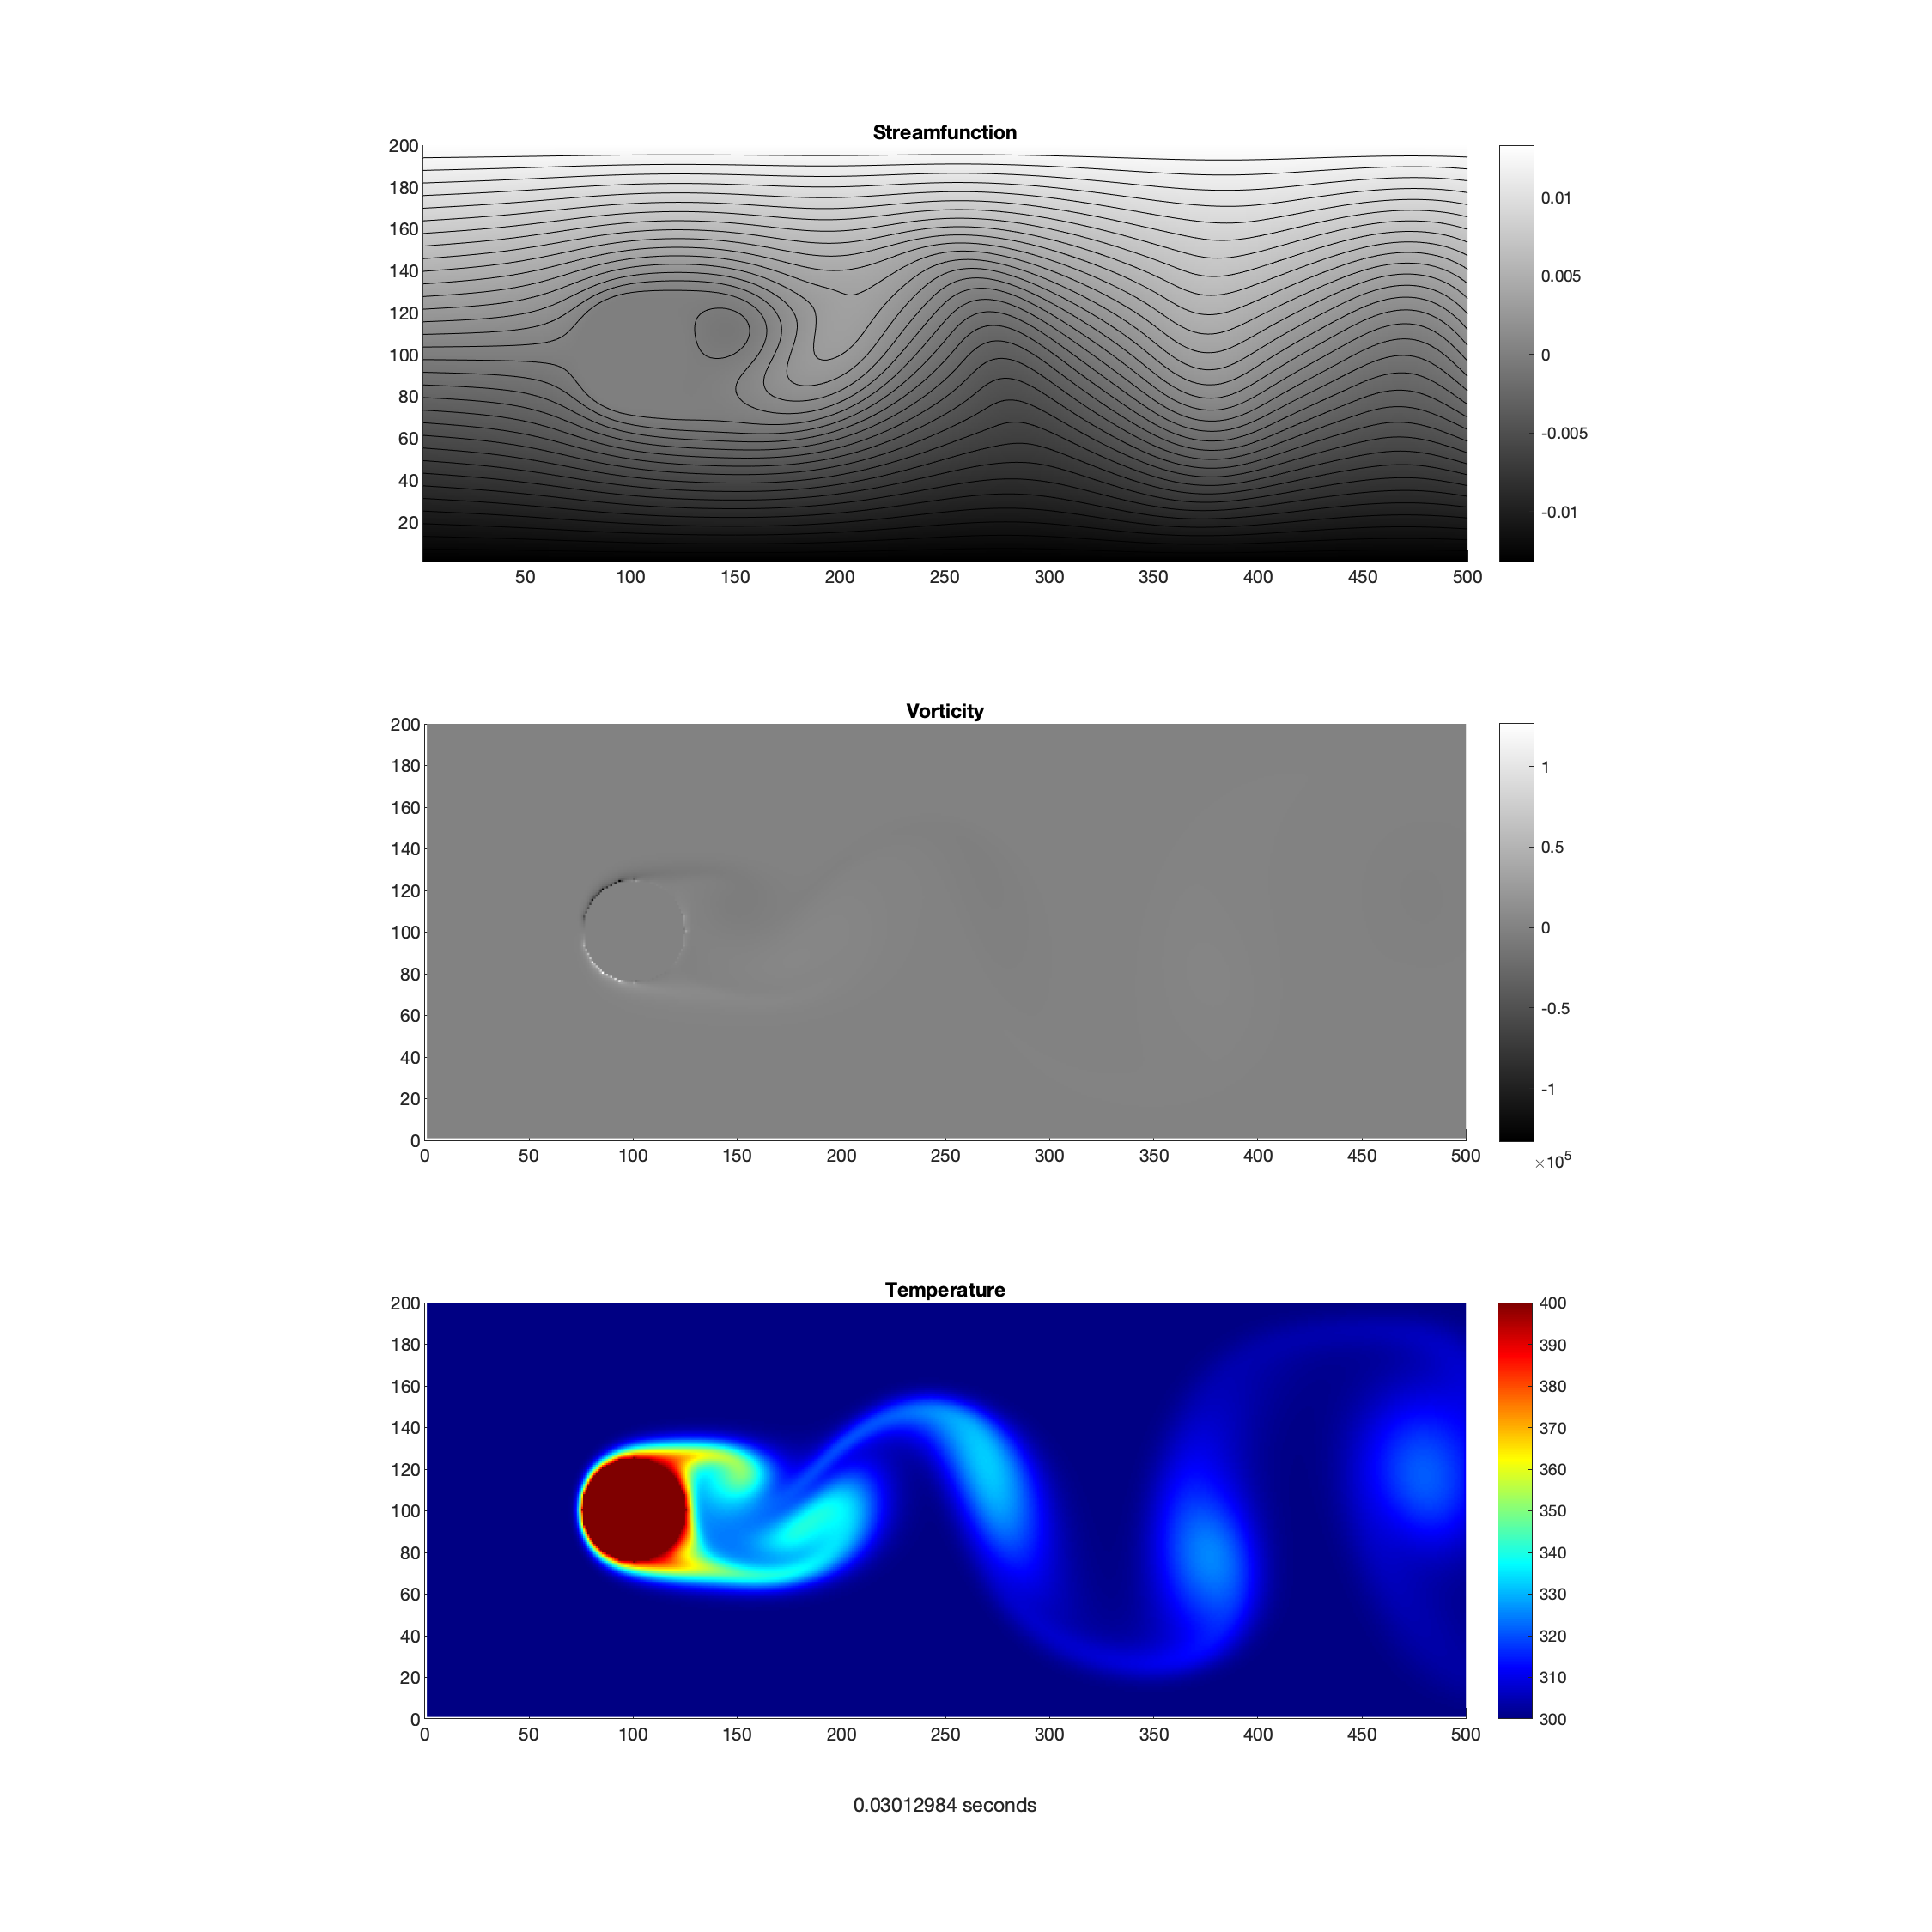
\includegraphics[width=\linewidth]{images/Final-Project-56550.png}
 \caption{Part 1 Simulation after 56,550 Time Steps}
\end{figure}

In the simulation for Part 1, the vorticies only start to form after around 10,000 time steps. Initially, the flow is symmetrical about the line y = 100. The vorticies start to form at the t = 0.0084s mark. After the vorticies form, they grow until the flow reaches dynamic equilibrium. From this point on, the flow does not change its behaviour. There is a small area of hot fluid around the cylinder.  
\pagebreak

\begin{figure}[h]
\centering
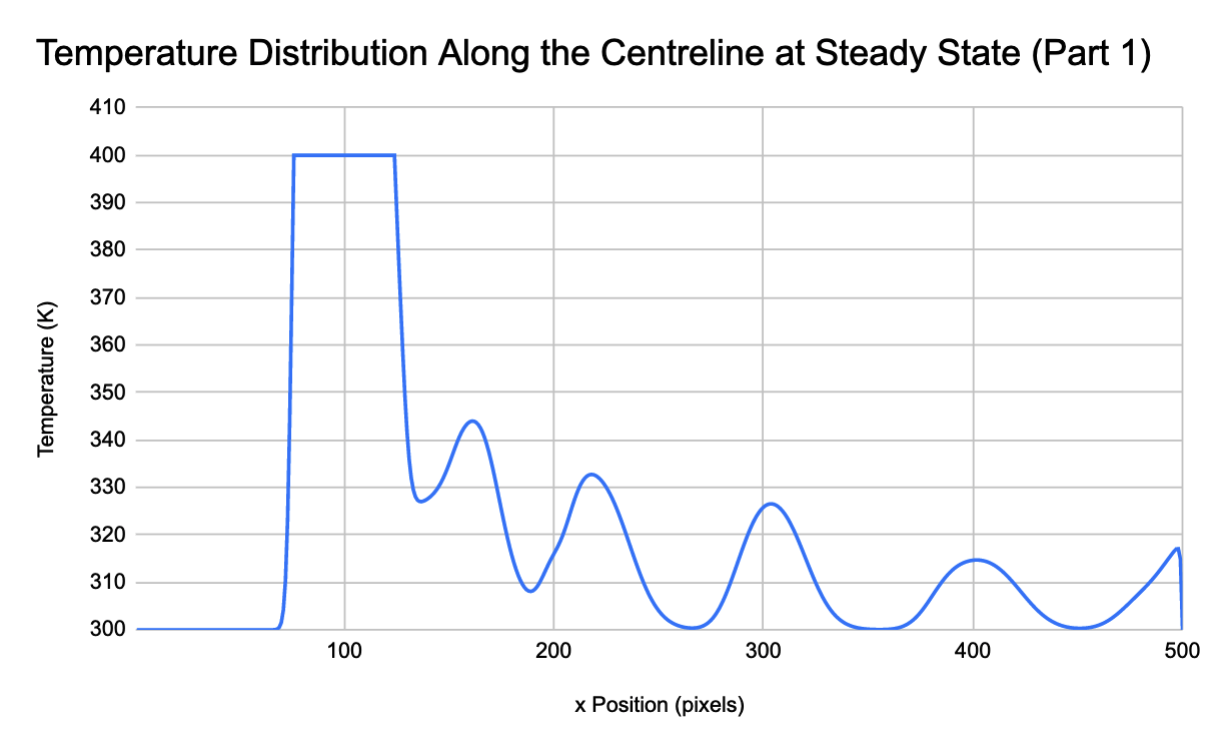
\includegraphics[width=0.7\linewidth]{images/Temp-Part-1.png}
 \caption{Temperature along Centerline at Steady State (Part 1)}
\end{figure}
\begin{figure}[h]
\centering
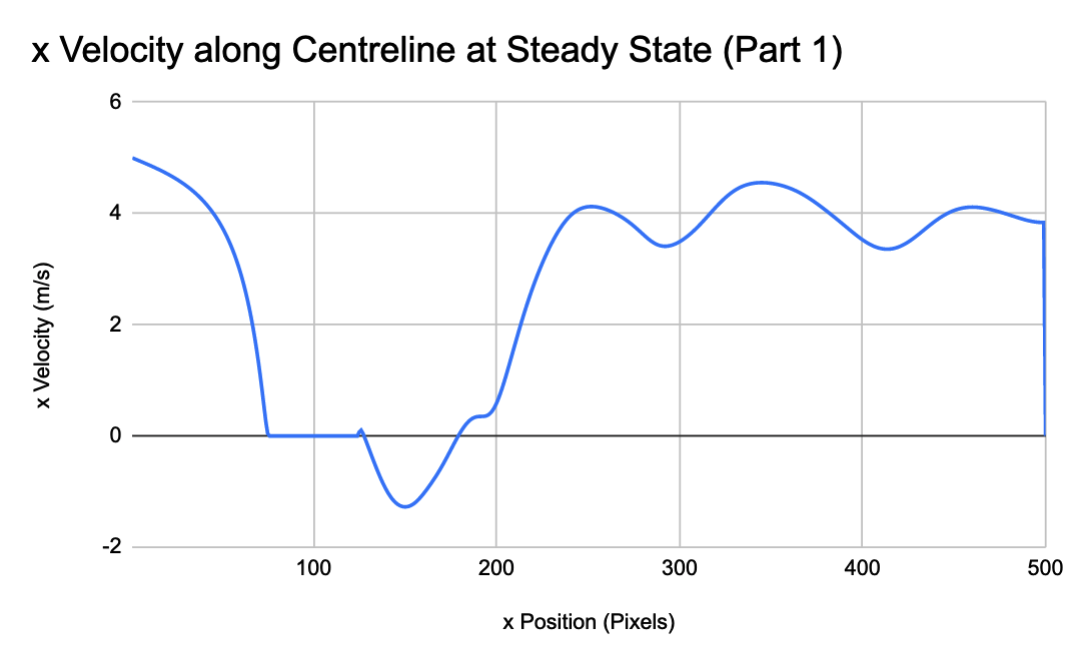
\includegraphics[width=0.7\linewidth]{images/xVel-Part-1.png}
 \caption{x Velocity along Centerline at Steady State (Part 1)}
\end{figure}


\clearpage

\subsection{Part 2} 

\begin{figure}[h]
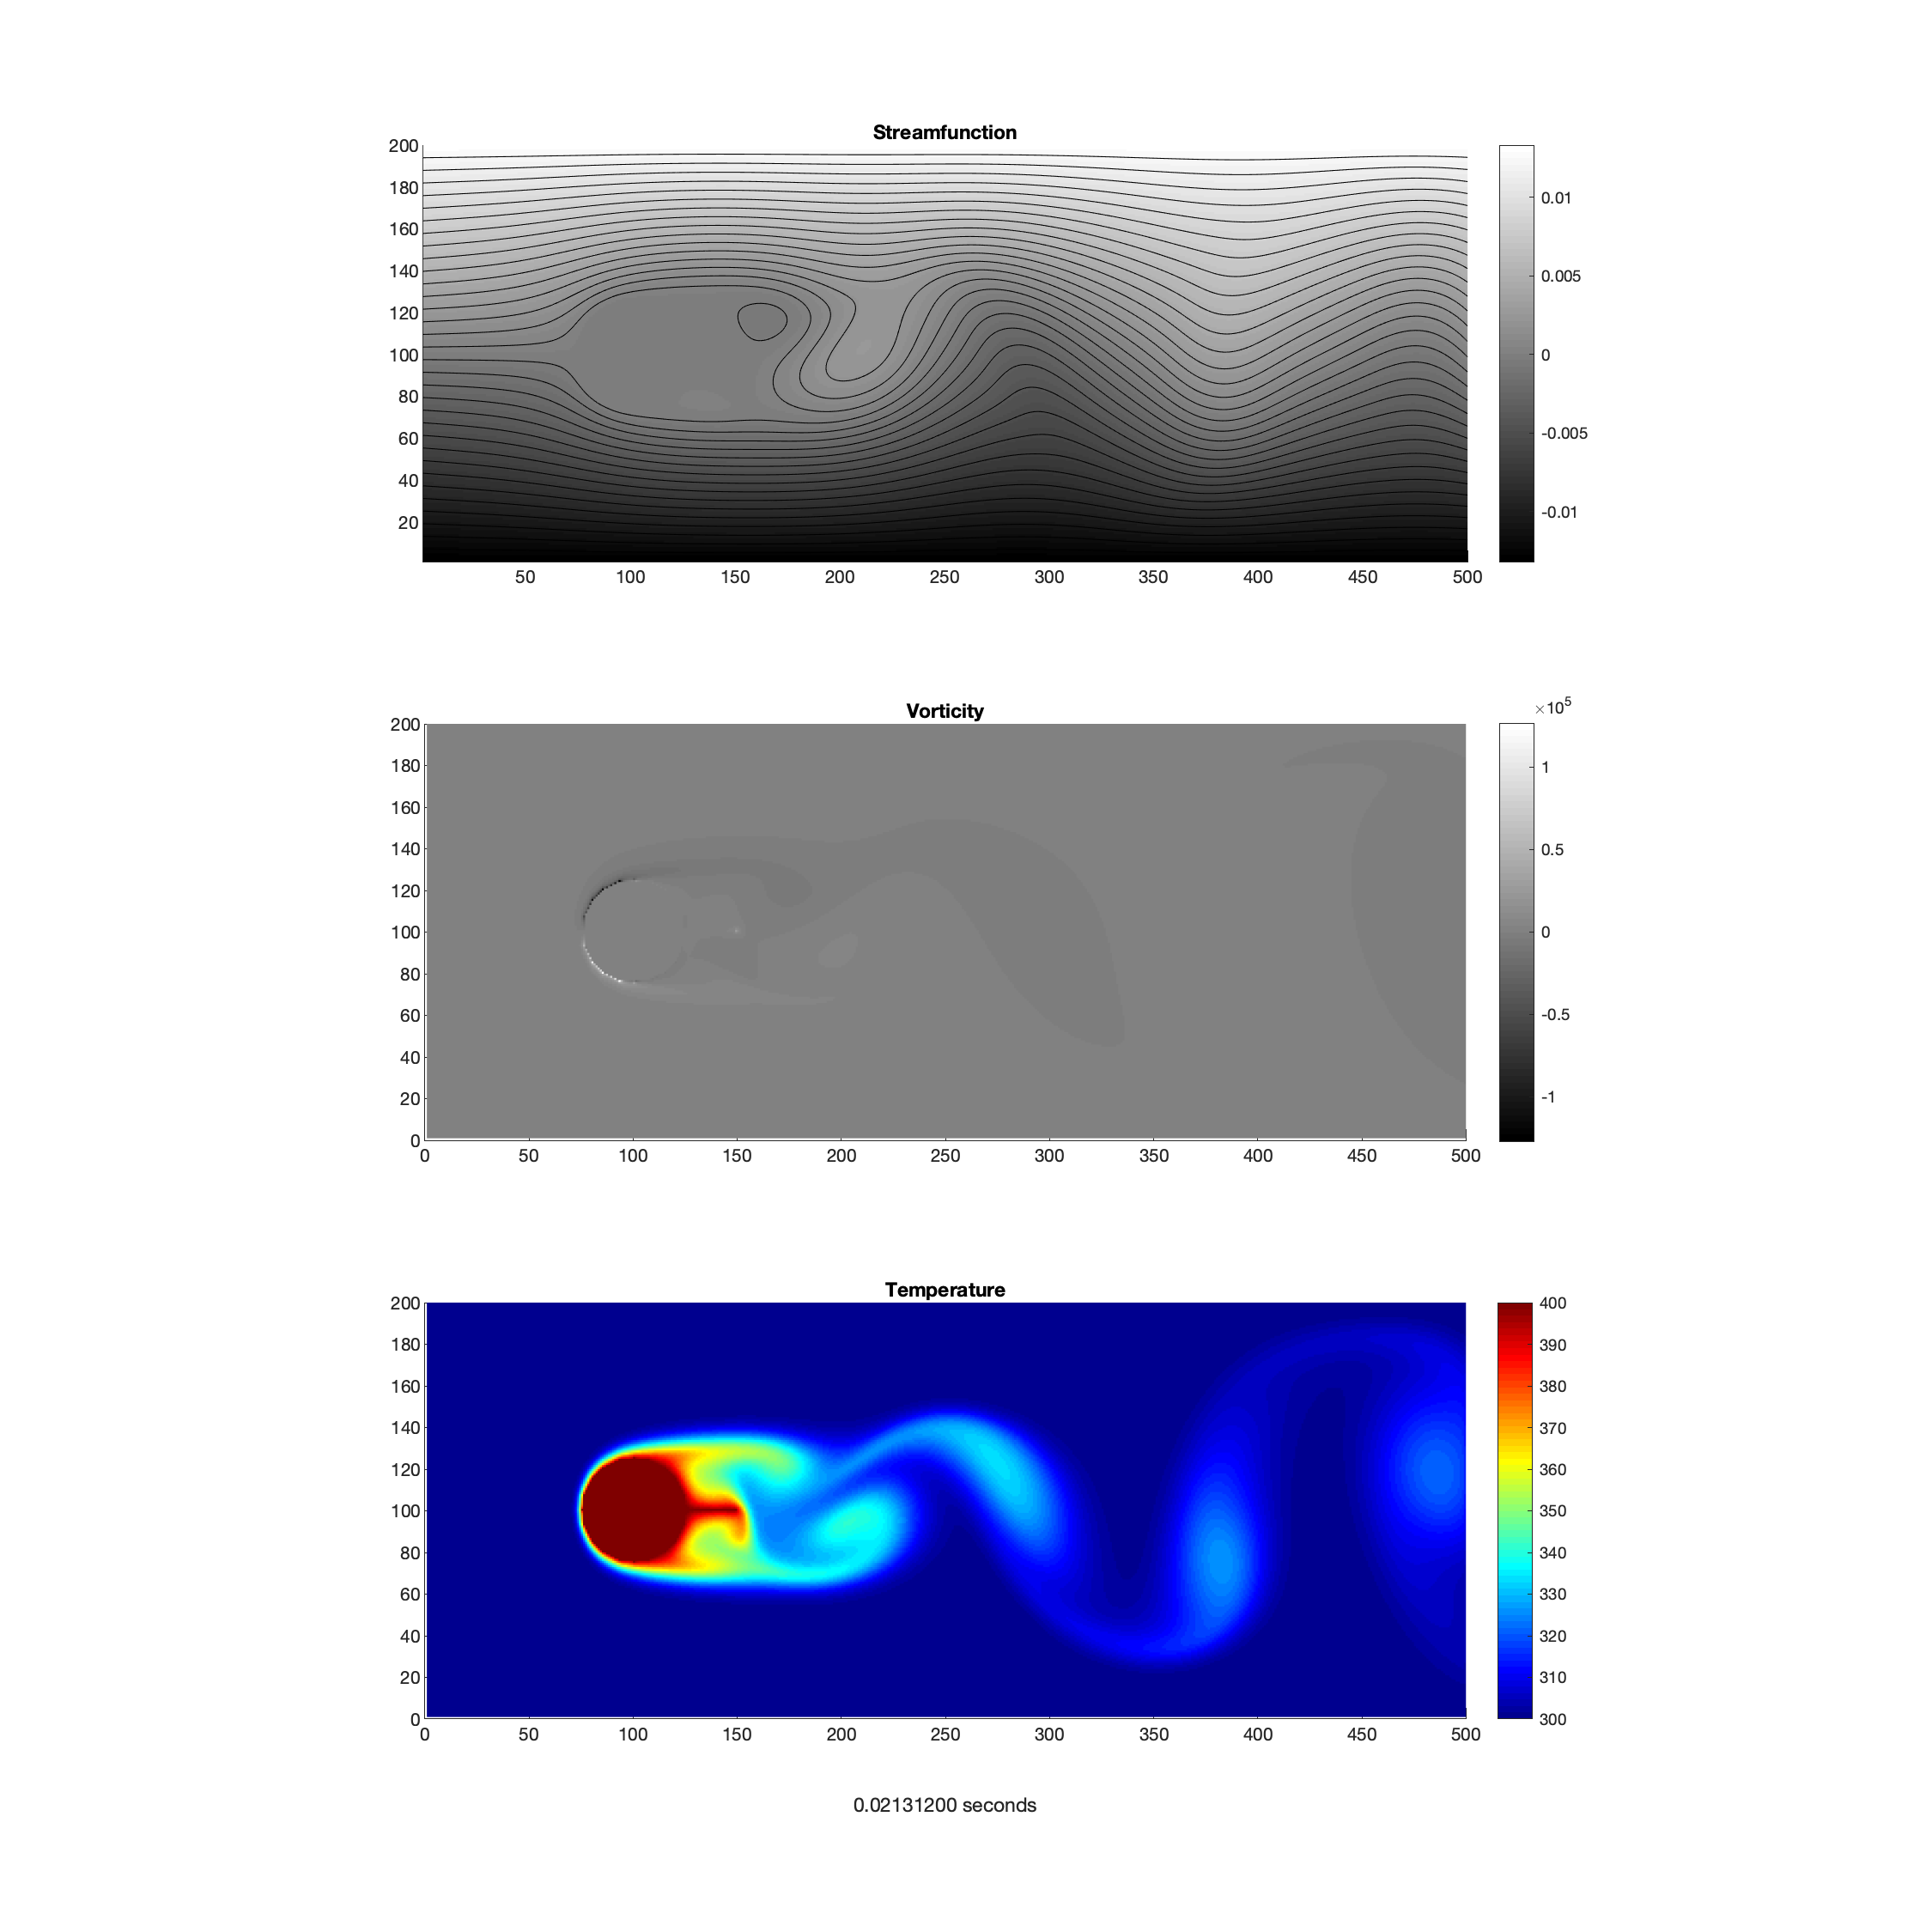
\includegraphics[width=\linewidth]{images/Part-2-Final-Project-40000.png}
 \caption{Part 2 Simulation after 40,000 Time Steps}
\end{figure}

In the part 2 simulation, the behavior is very similar to that of Part 1. Initially, the flow is symmetrical about the line y = 100. Vorticies start to form from the t = 0.0106s point. This is 0.0022s later than they form in Part 1. From here, they grow until they are fully developed where the flow reaches its dynamic equilibrium and remains constant in time from that point on. The main difference between this flow and Part 1 is that the vorticies are slightly smaller and they begin further downstream than they do in Part 1. From the vorticity plots, it can be seen that the vorticity in Part 2's flow fields is much more concentrated in the center of the shedding flow. This is seen in the contrast of the clockwise and counter-clockwise vorticities' colors (In Part 2: more white and black, in Part 1: more gray). The fin on the back of the cylinder in Part 2 has caused there to be a much more noticeably large area of hot fluid on the downstream side of the cylinder. 

\clearpage 

\begin{figure}
\centering
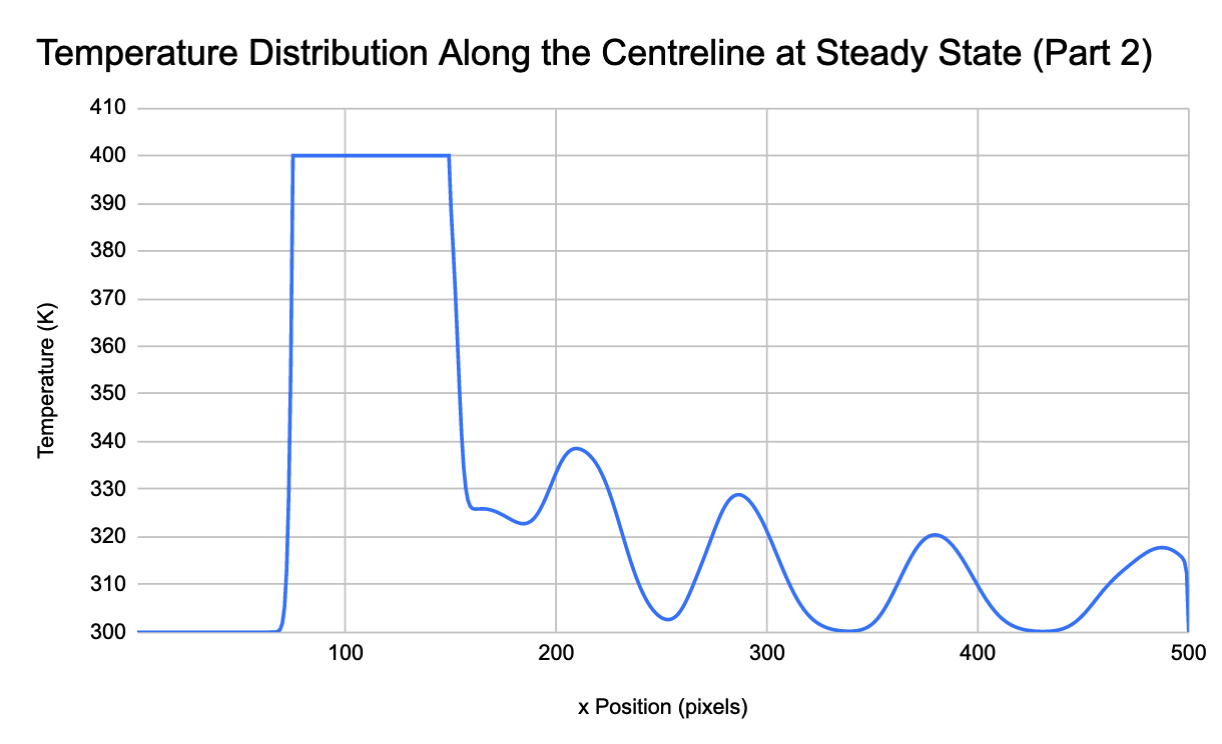
\includegraphics[width=0.7\linewidth]{images/Temp-Part-2.png}
 \caption{Temperature along Centerline at Steady State (Part 2)}
\end{figure}

\begin{figure}
\centering
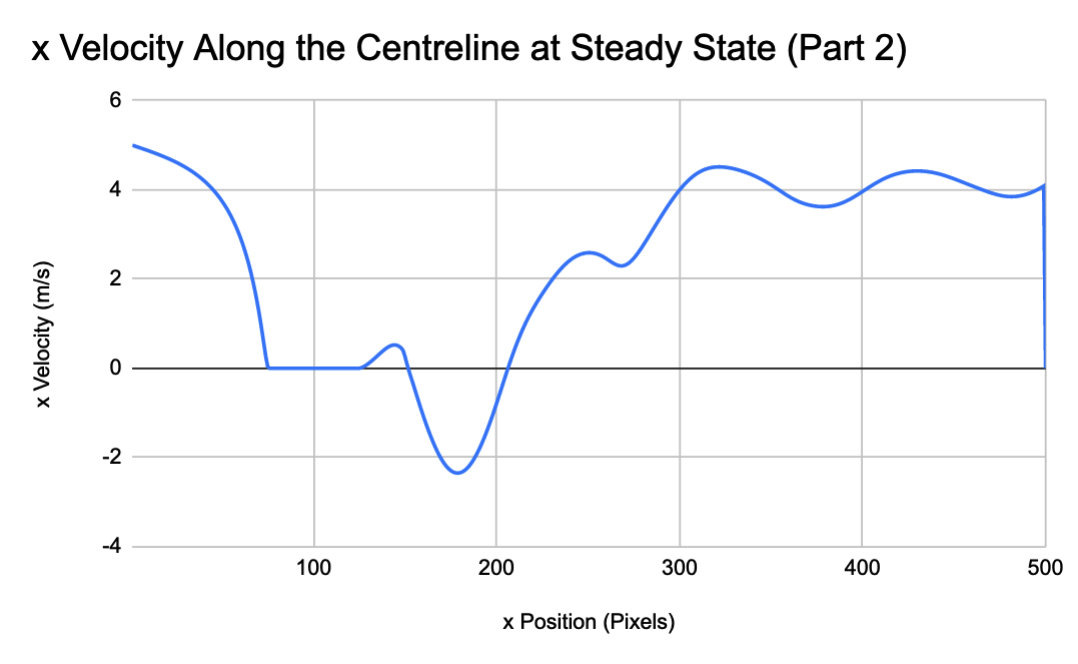
\includegraphics[width=0.7\linewidth]{images/xVel-Part-2.png}
 \caption{x Velocity along Centerline at Steady State (Part 2)}
\end{figure}











 
\clearpage